\documentclass[DIV15,a4paper]{scrartcl}

\usepackage{amsmath}
\usepackage{amsfonts}
\usepackage{algorithm}
%\usepackage{subfigure}
%\usepackage{subcaption}
\usepackage{setspace}
\usepackage[titletoc]{appendix}
\usepackage{tabularx}
\newcommand{\argmax}{\operatornamewithlimits{argmax}}

\usepackage{tikz}
\usetikzlibrary{positioning,shapes,shadows,arrows,calc}
\tikzstyle{component}=[rectangle, draw=black, rounded corners, fill=blue!40, drop shadow, text centered, anchor=north, text=white, minimum height=1cm]
\tikzstyle{arrow}=[->, thick]


\usepackage{graphicx}
\definecolor{Gray}{gray}{0.9}
\usepackage{scrpage2}
%\usepackage{graphicx}

\usepackage{datetime}

%\pagestyle{scrheadings}
%\ohead{D2.7 -- How to Design Self-aware Systems}
%\ihead{FP7-257906 EPiCS}
%\cfoot{Page \thepage\ of \pageref{LastPage}}

\usepackage{lscape}

\usepackage[colorlinks=true,
        linkcolor=black,
        citecolor=black,
        filecolor=black,
        urlcolor=black,
        bookmarks=true,
        bookmarksopen=true,
        bookmarksopenlevel=3,
        plainpages=false,
        pdfpagelabels=true]{hyperref}	% always as last package
\begin{document}

%%%%%%%%%%%%%%%%%%%%%%%%%%%%%%%%%%%%%%%%%%%%%%%%%%%%%%%%%%%%%%%%%%%%%%%%%%%%%
% Document start
%%%%%%%%%%%%%%%%%%%%%%%%%%%%%%%%%%%%%%%%%%%%%%%%%%%%%%%%%%%%%%%%%%%%%%%%%%%%%

%%%%%%%%%%%%%%%%%%%%%%%%%%%%%%%%%%%%%%%%%%%%%%%%%%%%%%%%%%%%%%%%%%%%%%%%%%%%%
\section{Background}
Self-Adaptive Software (SAS) is a special category of software that can change its own behaviors and structure in response to the dynamic and uncertain environment at runtime (e.g., changing workload) \cite{Lemos2013}. In the past decade, SAS has been widely applied in a range of application domains, including pervasive computing, robotics, service computing and cloud computing. The primary goal of SAS is to continually optimize some important, and possibly conflicted, non-functional attributes (e.g., performance, reliability, cost and energy),  thus their requirements can be better complied. Typically, SAS consists of two parts: an adaptable software and an adaptation engine that controls the adaptable software. Such fact does require the target software to be adaptable, i.e., it needs to have a set of well-defined interfaces for sensing and effecting. This is because in software engineering, there are many instances where the source code of the software is hidden or it cannot be changed at runtime. In addition, as stated by Welsh and Sawyer \cite{Welsh2008}, making a software adaptable may be the key condition of a solution, especially when the non-functional attributes and their priorities changes according to the environment.


\begin{figure}[h]
\centering
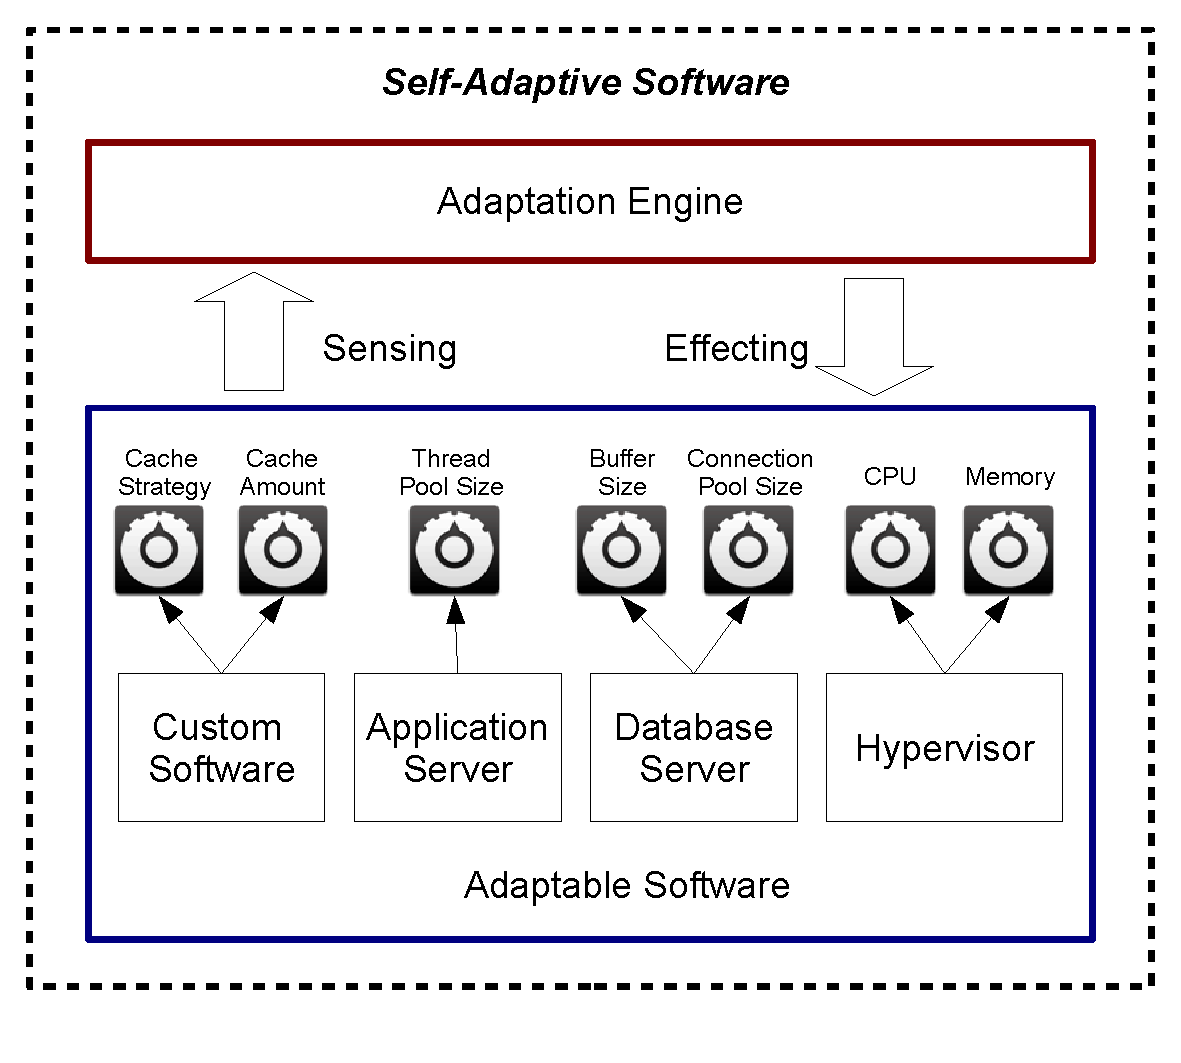
\includegraphics[width=10cm]{example.pdf}
\caption{An exampled architecture of SAS.}
\label{fig:arch}
\end{figure}

Figure \ref{fig:arch} shows a typical example of the architecture for SAS. A custom software is deployed and running on top of some other commercial off-the-shelf or free software, such as the application server, database server and hypervisor. Such software stack as a whole is actually an adaptable software, which consists of a set of well-defined interfaces. As we can see from the Figure \ref{fig:arch}, each of the software in the software stack could have one or more control knobs. For examples, the \textbf{Cache Strategy} in custom software can be configured as different modes, such as \emph{No-Cache}, \emph{Per-Application-Caching}, \emph{Per-Session-Caching} or \emph{Per-Request-Caching}, leading to different structure of its internal components; the application server can be adjusted to support a certain size of thread pool; and the hypervisor can be allocated with different amount of memory. Depending on the changing environment, all these control knobs and their interplay can cause different and significant impact to the non-functional attributes of the adaptable software. The decision of those control knobs can only be effectively made at runtime, since the environment changes and the sensitivity of non-functional attributes to those control knobs are often not known at design time. As the environment changes on-the-fly, optimizing the SAS architecture aims to search the right combination of control values that achieves the best non-functional performance. Although in Figure \ref{fig:arch}, we only illustrate an exampled architecture with 7 control knobs, it can still imply a complicated situation: suppose that there are 4 options for \textbf{Cache Strategy} and 20 options for each of the rest control knobs; and that there are no dependencies or mutual exclusions exist between them, then this has already given us a search space of $2.56 \times 10^8$ possible adaptation decisions. Consequently, optimizing SAS architecture at runtime requires novel algorithm to efficiently and effectively perform the computational search.

\section{How to effectively optimize SAS architecture at runtime and mitigate the effects of requirements uncertainty? (working with Ke)}

\subsection{The problem 1}

Majority of the work for optimization SAS architecture has been relying on weighted aggregation (usually weighted sum) of non-functional objectives \cite{Elkhodary:2010} and \cite{Esfahani:2011}, in which the weights are specified by users. However, the the well-know drawback of this approach is that it may be difficulty for a software engineer to specify weights and the result only provide partial information of the trade-off surface. There are few instances where evolutionary multi-objective algorithms (mainly NSGA-II) are used, but they are specific to an application domain of SAS, e.g., cloud \cite{2014-eplison-GA-weigh-h-scaling-2014}, \cite{E3-R-extended}. Evolutionary multi-objective optimization for SAS architecture in general has been limited. As a result, there are plenty of opportunities for exploring more advance evolutionary multi-objective optimization to this problem.

\subsection{Our proposal 1}

Our proposal is to explore better evolutionary multi-objective algorithm to the problem of SAS architecture optimization. In particular, we aim to produce knee solutions for the problem. We might start from the scenarios where objective number is less than 3, and we can explore many objective optimization in the future. In particular, we have the following research questions:

\begin{itemize}

\item How to better handle the mixed control variables (e.g., categorical, discrete and integer variables) in the adaptable software?

\item How to design/select the operator and how to produce individual given mixed control variables?

\item Considering knee points in the optimization process v.s. considering them after the optimization, which one is better?

\item Whether the proposal approach is better than existing weighted sum optimizations and NSGA-II?

\end{itemize}


\subsection{The problem 2}

For any SAS, stakeholders often specify a set of requirements on the non-functional attributes, representing their satisfactions/expectation on the SAS, e.g., \emph{the response time of the SAS should be less than 2 seconds}. These requirements would be used as (usually soft) constraints on the adaptation engine of SAS and they may be changed at runtime, as requested by the stakeholders. However, the requirements exhibit \emph{uncertainty}, by which we refer to the rationality of requirements is uncertain, hence they may be unrealistic and misleading. This is because the requirements given by stakeholders are highly subjective and depending on their domain knowledge/assumptions, hence inevitably prone to uncertainty in the rationality of those requirements. In addition, engineers may also provide requirements for certain non-functional attributes that cannot be easily monitored. For instance, the maximum memory consumed by the adaptable software and its best possible performance are properties that may be available from the software's source code, but not easily obtainable through runtime monitoring. Consequently, engineers may influence the requirements based on their past experience, which again introduces uncertainty. The problem becomes even more complex when the non-functional attributes requires trade-offs, i.e., they are conflicting. 

Optimization for SAS architecture can be formulated in two ways: constraint satisfaction and objective optimization. However, the requirements (constraints) play an integral roles in both formalizations, hence they may affect the optimization in the following ways if their uncertainty is not properly handled:

\begin{itemize}

\item If the given requirements are too good, the optimization of SAS architecture may be struggle to find feasible decisions and thus difficult to converge to optimal result(s), as the requirements introduce too much pressure in the search process.

\item If the given requirements are too bad, the requirements may not produce enough search pressure and thus losing the point of having those requirements.

\end{itemize}

Therefore, how to handle the uncertainty in stakeholders' requirements is a significant problem and it has been identified as one of the key research challenges for engineering SAS \cite{Cheng2009} \cite{Esfahani:2011}.


Most of the work (e.g., the FUSION \cite{Elkhodary:2010} and \cite{Esfahani:2011}) on SAS architecture optimization assume that the requirements are always be rationally given, which is unrealistic. On the other hand, existing efforts for dealing with requirements uncertainty has been focusing on \emph{top-down} manner. Specifically, traditional work try to address the problem by designing a methodology that can help stakeholders when specifying requirements \cite{1317482} at design time. However, this requires a lot assumptions, e.g., each non-functional attribute can be considered independently. In addition, such an approach cannot deal with the uncertainty caused by requirement changes at runtime. More recently, the community has been using Model@runtime paradigm to 'reflect' the requirements at runtime \cite{Song2013}. In those approaches, the requirements are continually reasoned at runtime based on monitoring of the SAS. The aim is to correct those irrational requirements, which might be too good or too bad, after a period of time; and to handle requirements changes. Nevertheless, the drawback is obvious: it may need quite a few adaptation cycles for the requirements to stabilize and the initial quality of requirement can significantly affect the process. All these approakch are called \emph{top-down} because they try to reason about the requirements before they are used in the subsequent optimization process.

\subsection{Our proposal 2}

Instead of tackling the problem in the traditional  \emph{top-down} manner, we try to resolve it via a  \emph{bottom-up} way: we aim to develop an underlying optimization algorithm that is resilient to the requirements uncertainty. That is to say, even when the given requirements are too good or too bad, we anticipate that the algorithm can still produce optimal or near-optimal results. By doing so, we free the stakeholders and engineers from the tedious assumptions and complicated requirements elicitation/negotiations process, which could in turn, save development effort. In addition, tackling the problem from a \emph{bottom-up} manner eliminates the need of another complex runtime process (i.e., Model@runtime). At this stage, we aim to answer three research questions:

\begin{itemize}

\item Assuming that rational requirements are given, how to consider those requirements in SAS architecture optimization?

\item Optimizing with rational requirements v.s. optimizing without (i.e., the approach from proposal 1), which one is better?

\item Considering rational requirements in the optimization process v.s. considering them after the optimization, which one is better?

\item Removing the assumption of rational requirements. Now the question becomes: how to formulate the problem and design the corresponding optimization algorithm that can mitigate requirements uncertainty?

\item How does the algorithm perform when compared with others under irrational requirements?

\end{itemize}

\subsection{The problem 3}

Existing work for optimizing SAS architecture has assumed static optimization, i.e., there is an isolated optimization problem at each time step during the entire runtime life cycle. Given the runtime nature of the SAS architecture optimization problem, changes can occur anytime during the optimization, thus turning the classic static optimization into dynamic optimization might yield additional benefits. However, new challenges and considerations arise.

\subsection{Our proposal 3}

Our proposal is to model SAS architecture optimization as a dynamic optimization problem and propose related approach to solve it. We have the following research questions:

\begin{itemize}

\item How to model the dynamics in the SAS architecture optimization problems? e.g., dynamics in workloads and the sensitivity of non-functional attributes to control variables?

\item How to design the corresponding optimization algorithm to cope with dynamics? What dynamics handling strategy to use?

\item Dynamic optimization v.s. static optimization, what are the added values?

'\end{itemize}



\section{When to trigger optimization and adaptation in SAS architecture? (working with Shuo)}

\subsection{The problem}

Adaptations in SAS architecture occurs continually and it is often driven by the result of architecture optimization. This would therefore rise the questions of \emph{when} or \emph{how often} to adapt the SAS. It is again another dilemma: too frequent adaptations may generate large overhead as the optimization/adaptation process does not comes as free. On the other hand, too rare adaptations might not be useful for the SAS to response to the changes in environment. This problem is also one of the key research challenges in the field \cite{Brun2013}.


A generally recognized approach in the field is to trigger optimization/adaptation on-demand \cite{Elkhodary:2010}\cite{Esfahani:2011}. That is to say, the SAS will adapt once the requirements of non-functional attributes are violated (or some safe thresholds of requirements are violated). Such an approach can work in either reactive or proactive manner, for example, optimization/adaptation can be triggered when the violations have already occurred or they are predicted to occur very soon. However, this approach can be still problematic when:

\begin{itemize}

\item The violation is trivial.

\item The payoff after the optimization is trivial under current circumstance.

\end{itemize}

\subsection{Our proposal}

We intend to adopt online machine learning and concept drift technique to capture the correlation between requirement violation, the benefits and cost after optimization/adaptation. Upon the occurrence of requirement violation, we aim to establish model(s) to assist more systematic reasoning about whether to trigger optimization in the SAS architecture. In this way, we anticipate that the proposed approach will reduce overhead in the adaptation engine and potentially improve stability of the SAS architecture. At this stage, we aim to answer three research questions:

\begin{itemize}

\item What are the important features that should be consider in the learned models?

%\item How to quantify the payoff for optimization/adaptation and the significance of requirements violation?

\item How to reason about and make trade-off between optimization/adaptation cost and payoff when optimization in runtime architecture? (I am discussing with Rami about using Technical Debt to this research question)

\item Whether it is beneficial to continually track the changes in the models using concept drift (e.g., sudden changes in workload) and how to achieve such?
\end{itemize}

\section{About evaluation}

Currently there are quite a few existing benchmark software exist in the community of Performance Engineering, Requirement Engineering and Software Engineering for Self-Adaptive Software Systems. Among others, the most popular ones are Znn.com \footnote{http://adaas.dei.uc.pt/adaas/resources/znn.com}, RUBiS \footnote{http://rubis.ow2.org/}, TPC \footnote{http://www.tpc.org/tpcw/} and GridStix \footnote{Hughes, D., Greenwood, P., Coulson, G., Blair, G.: GridStix: supporting flood prediction using embedded hardware and next generation grid middleware. World of Wireless, Mobile and Multimedia Networks (2006)}. We plan to evaluate our approach based on one or more of the above. The evaluation metrics can be the achieved non-functional results and their compliance with respect to requirements. Additionally, the metrics (e.g., hypervolumn, GD and IGD) in multi-objective optimization community can be also applied.

In a later stage of dissemination, we intend to integrate our work with an open source software. Currently, I am thinking of choosing one from the Apache Software Foundation as it is well recognized as one of the largest open source software corporation.

\bibliography{references}
\bibliographystyle{abbrv}

\end{document}
